\documentclass[11pt,a4paper]{article}
\usepackage[T1]{fontenc}
\usepackage{lmodern}
\usepackage{float}
\usepackage[margin=2.2cm]{geometry}
\usepackage{booktabs,tabularx,enumitem,xcolor,array,graphicx}
\usepackage[hidelinks]{hyperref}

\setlist{nosep}
\newcommand{\svc}[1]{\texttt{#1}}
\newcolumntype{Y}{>{\raggedright\arraybackslash}X}

\begin{document}

\section{Access, Users and Passwords}

For security and centralized configuration, credentials are injected with Docker secrets mounted at \texttt{/run/secrets}. For testing purposes within this laboratory setup, default passwords are standardized to \texttt{groupH}, the only exception is the Moodle administrator, because Moodle refuses passwords that do not follow its policy (upper and lower case, digit, and symbol).

\subsection{Web Addresses}

\begin{table}[H]
\centering\small
\begin{tabularx}{\textwidth}{llXl}
\toprule
Service & Local (\texttt{compose.yml}) & Production (\texttt{production.yml}) & Auth \\
\midrule
Reviews application & \texttt{http://app.localhost:8080} & \texttt{https://app.localhost} & Public \\
Moodle (Atenea) & \texttt{http://lms.localhost:8080} & \texttt{https://lms.localhost} & Required \\
Grafana & \texttt{http://grafana.localhost:8080} & \texttt{https://grafana.localhost} & Required \\
Mailpit & \texttt{http://mail.localhost:8080} & \texttt{http://mail.localhost:8080} & Public \\
\bottomrule
\end{tabularx}
\caption{Deployed web endpoints and authentication requirements.}
\label{tab:endpoints}
\end{table}

\begin{figure}[H]
\centering
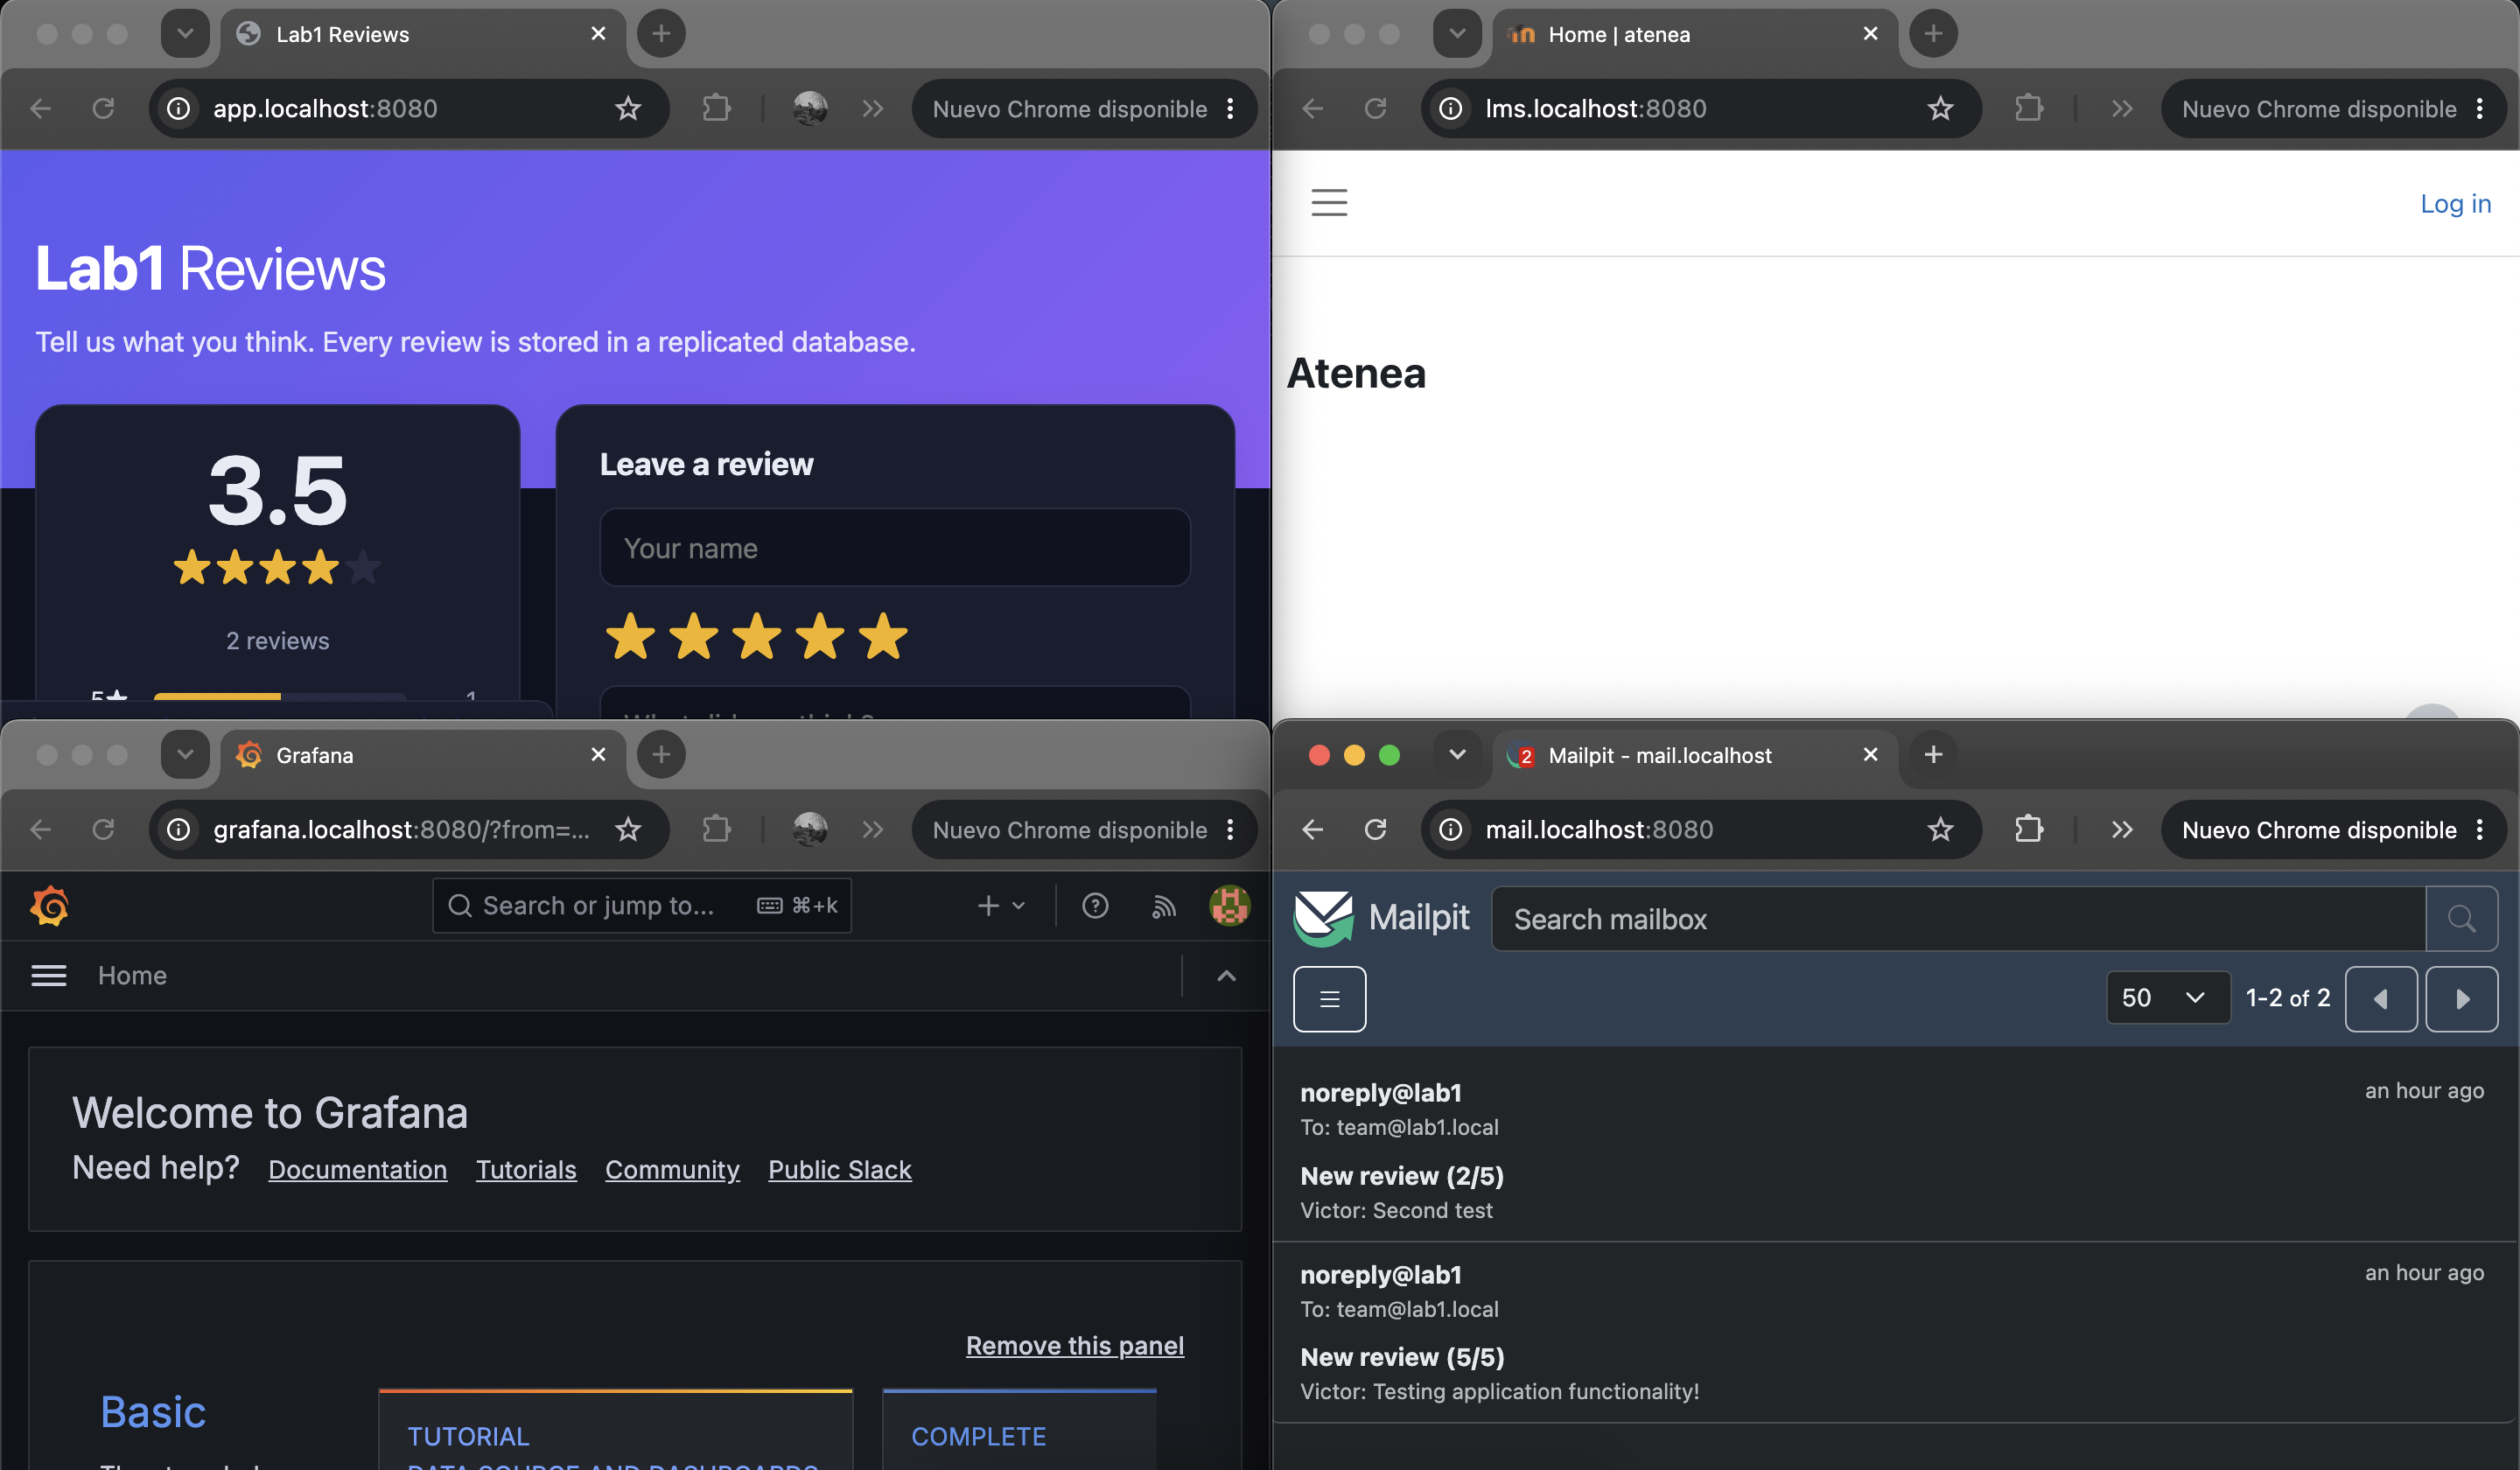
\includegraphics[width=0.85\textwidth]{screenshot4webs.png}
\caption{Running deployment of the web addresses.}
\label{fig:app_preview}
\end{figure}

\subsection{Users and Passwords}

Table~\ref{tab:credentials} shows the service credentials, secret files, and the configured database access scopes.

\begin{table}[H]
\centering\small
\begin{tabularx}{\textwidth}{lllY}
\toprule
\textbf{Service} & \textbf{User} & \textbf{Password} & \textbf{Secret File} \\
\midrule
Grafana & \texttt{admin} & \texttt{groupH} & \texttt{grafana\_admin\_password} \\
Moodle & \texttt{admin} & \texttt{groupH-2026} & \texttt{moodle\_admin\_password} \\
PostgreSQL (Patroni) & \texttt{postgres} & \texttt{groupH} & \texttt{pg\_admin\_password} (Internal HA management) \\
PostgreSQL (App) & \texttt{app} & \texttt{groupH} & \texttt{app\_db\_password} (Owner of \texttt{app} DB) \\
PostgreSQL (Grafana) & \texttt{grafana} & \texttt{groupH} & \texttt{grafana\_db\_password} (Owner of \texttt{grafana} DB) \\
PostgreSQL (Replication) & \texttt{replicator} & \texttt{groupH} & \texttt{replicator\_password} \\
PostgreSQL (Backup) & \texttt{backup} & \texttt{groupH} & \texttt{backup\_db\_password} (\texttt{pg\_read\_all\_data}) \\
PostgreSQL (Metrics) & \texttt{exporter} & \texttt{groupH} & \texttt{exporter\_db\_password} (\texttt{pg\_monitor}) \\
MariaDB (Moodle) & \texttt{moodle} & \texttt{groupH} & \texttt{moodle\_db\_password} \\
MariaDB (Auxiliary) & \texttt{backup}, \texttt{exporter} & \texttt{groupH} & Shared secrets (Read-only access) \\
Backup Encryption & --- & \texttt{groupH} & \texttt{backup\_passphrase} (AES-256-CBC) \\
Self-signed TLS key & --- & \texttt{groupH} & \texttt{CERT\_PASSWORD} \\
Feeder API & --- & \texttt{groupH} & \texttt{feed\_token} (Bearer Token) \\
\bottomrule
\end{tabularx}
\caption{System account roles and Docker secret mappings.}
\label{tab:credentials}
\end{table}


\section{Data Management and Backups}
\label{sec:backup}

To avoid database corruption caused by network disruptions or file-locking conflicts, transactional DBMS files are stored directly on local node drives rather than over NFS.

\begin{table}[H]
\centering\small
\begin{tabular}{lll}
\toprule
\textbf{Data Target} & \textbf{Volume Name} & \textbf{Physical Node Location} \\
\midrule
PostgreSQL Cluster \& etcd & \texttt{pg-1..3}, \texttt{etcd-1..3} & Local disk (\texttt{app1}, \texttt{app2}, \texttt{stats}) \\
MariaDB \& NFS Root & \texttt{moodle-db}, \texttt{nfs-data} & Local disk (\texttt{atenea}) \\
Moodle Data \& Certificates & \texttt{moodledata}, \texttt{certs}, \texttt{acme} & NFS Storage (\texttt{atenea}) \\
Encrypted Backups & \texttt{backups} & Dedicated disk (\texttt{backup}) \\
Prometheus Replicas & Anonymous volumes & Local disk (\texttt{stats}, \texttt{backup}) \\
Redis Cache & In-Memory & Replicated RAM \\
\bottomrule
\end{tabular}
\caption{Physical storage distribution across Swarm nodes.}
\label{tab:storage_layout}
\end{table}

The backup service operates on a dedicated host isolated from core application nodes. Scheduled daily at 03:30, the pipeline performs:
\begin{enumerate}
    \item \textbf{PostgreSQL Dump}: Uses \texttt{pg\_dump -Fc} routed to read-only replicas (\texttt{db:5433}) under the \texttt{backup} role to prevent load on the HA leader.
    \item \textbf{MariaDB Dump}: Executes \texttt{mariadb-dump --single-transaction} for transactional consistency.
    \item \textbf{Moodle Data Storage}: Archives \texttt{moodledata} while stripping volatile session and cache directories.
    \item \textbf{Encryption \& Integrity}: Encrypts files using OpenSSL AES-256-CBC (PBKDF2) with the secret passphrase and generates matching \texttt{SHA256SUMS}.
\end{enumerate}

Backups are initially written with a \texttt{.partial} suffix and atomic-renamed upon completion, and retention is configured for 14 days.

An automated integrity check runs every Sunday (and on demand with \texttt{docker exec <backup> /restore-test.sh}). The routine verifies checksums, decrypts archives, restores dumps into temporary containerized DBMS instances, and validates recovered row and table counts. Test outcomes are exported to Prometheus (\texttt{backup\_restore\_test\_ok}).


\section{Observability}
\label{sec:obs}

Prometheus uses DNS service discovery (\texttt{tasks.<service>}) so scaled replicas are scraped without manual changes. Dashboards are provisioned declaratively via Git, where Grafana visualizes node metrics alongside custom ratings using the Infinity plugin. Additionally, Prometheus alerting rules (\texttt{rules.yml}) flag offline endpoints, replication delays, missing cluster leaders, and backup failures. Table~\ref{tab:obs} summarizes the metric sources and monitored targets.

\begin{table}[H]
\centering\small
\renewcommand{\arraystretch}{1.2}
\begin{tabularx}{\textwidth}{@{}>{\raggedright\arraybackslash}p{3.5cm}>{\raggedright\arraybackslash}p{3.5cm}Y@{}}
\toprule
\textbf{Metric Source} & \textbf{Monitored Target} & \textbf{Key Operational Indicators} \\
\midrule
\texttt{core} & Python Microservice & Requests/sec, posted reviews, Redis cache hit/miss ratio \\
Nginx Exporter & Frontend Proxy & Active connections, throughput per replica \\
Postgres Exporter / Patroni & PostgreSQL Nodes & Connection pool, transactions, replication lag, leader status \\
Redis Exporter & Cache Instances & Master/Replica role, memory consumption, hit ratio \\
MySQLd Exporter & MariaDB Instance & Active threads, queries per second (QPS) \\
Blackbox Exporter & Web Endpoints & Availability and HTTP response latency for Moodle/Grafana/App \\
cAdvisor \& Node Exporter & Host Nodes & Node-level CPU, RAM usage, and container resource limits \\
Backup Exporter (9199) & Backup Service & Last execution age, duration, archive size, restore status \\
\bottomrule
\end{tabularx}
\caption{Observability exporters and monitored metrics.}
\label{tab:obs}
\end{table}

Figure~\ref{fig:grafana_dashboard} presents the main Grafana overview dashboard after simulating application traffic generated by user interactions with the reviews app.

\begin{figure}[H]
\centering
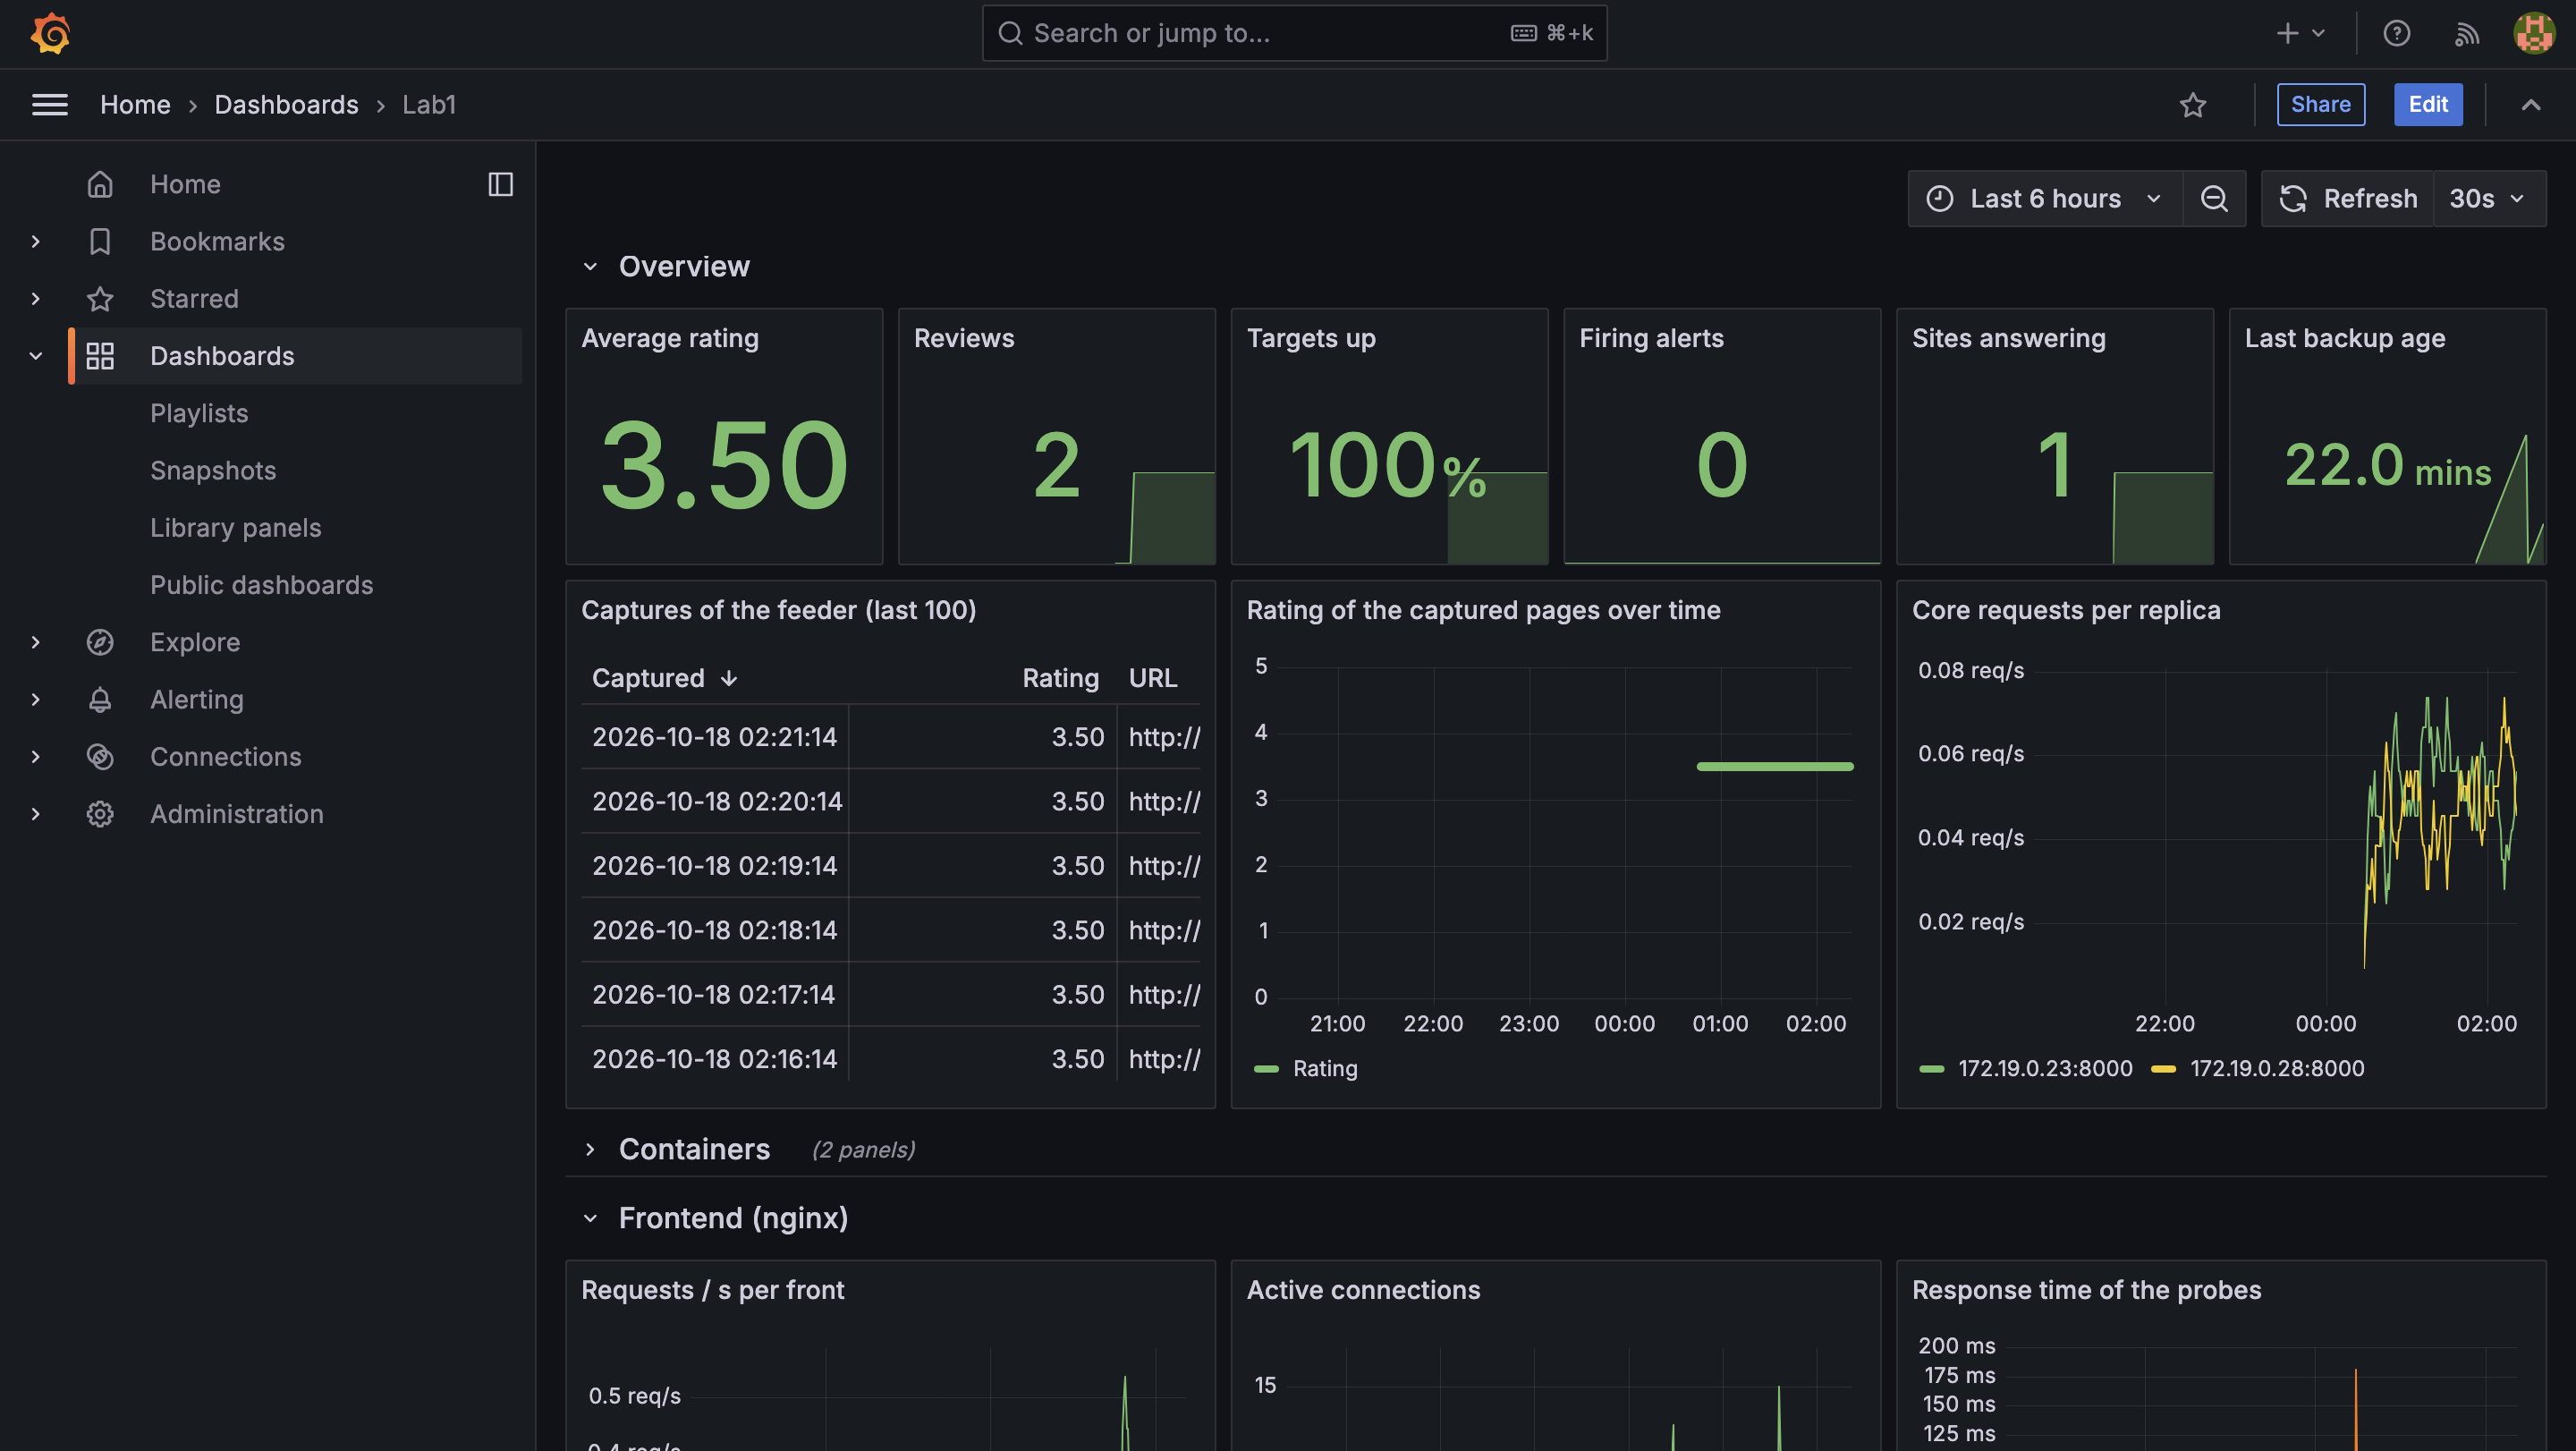
\includegraphics[width=0.95\textwidth]{grafana_dashboard.png}
\caption{Grafana monitoring dashboard.}
\label{fig:grafana_dashboard}
\end{figure}


\section{Security}

\begin{itemize}
    \item \textbf{Traffic Control}: Only Nginx exposes external ports ($80/443$). All traffic is forced through TLS 1.2/1.3 with HSTS enabled. Internal microservices remain isolated.
    \item \textbf{Least-Privilege Database Access}: Database owners (\texttt{app}, \texttt{grafana}) are restricted to their respective databases. The \texttt{replicator} user is confined to replication streams, and global \texttt{CONNECT} rights are revoked from \texttt{PUBLIC}.
    \item \textbf{Encrypted Inter-Node Communication}: Secrets are mounted in-memory at \texttt{/run/secrets}. Overlay networks utilize IPsec encryption, segregating individual application stacks.
    \item \textbf{Metrics Isolation}: Metric endpoints (\texttt{/metrics}) are blocked at the proxy layer, preventing external exposure.
\end{itemize}

\end{document}